% Enrique Acosta
% 2021

\documentclass[border=2pt, tikz]{standalone}
\usepackage{pgfplots}
\pgfplotsset{compat=1.17}
\usetikzlibrary{calc}

\begin{document}

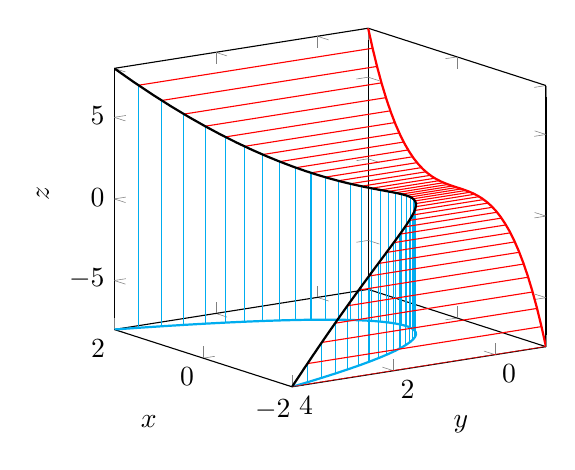
\begin{tikzpicture}%
\begin{axis}%
[ scale=0.8
, view={235}{15} % {rotation angle}{elevation angle}
, xlabel=$x$
, ylabel=$y$
, zlabel=$z$
, zmin=-8
, zmax=8
]

% Parabola and cubic shadow curves
\addplot3%
[ 
, samples=40
, samples y=0
, thick 
, cyan 
, domain=-2:2
, variable=\t
] ({t},{t^2},{-8});

\addplot3%
[ 
, samples=40
, samples y=0
, thick
, red 
, domain=-2:2
, variable=\t
] ({t},{-1},{t^3});


%  Lines
%  pgfplots cannot handle a \foreach commands inside the {axis} environment, so the draw commands need to have the foreach inside of them. See also pgfplotsinvokeforeach.
\draw [cyan] foreach \a in {-2,-1.9,...,2} {
({\a}, {(\a)^2}, {(\a)^3}) --  ({\a}, {(\a)^2}, -8)
};

\draw [red] foreach \a in {-2,-1.9,...,2} {
({\a}, {(\a)^2}, {(\a)^3}) -- ({\a}, -1, {(\a)^3})
};

% Twisted cubic
\addplot3%
[ 
, samples=51
, samples y=0
, thick
, black 
, domain=-2:2
, variable=\t
] ({t},{t^2},{t^3});

\end{axis}
\end{tikzpicture}

\end{document}